%% Elsevier elsarticle template for NIM-A submission
%% Numeric-reference version

\documentclass[preprint,12pt]{elsarticle}
% If the editor requests a double-spaced review version, switch to:
% \documentclass[preprint,review,12pt]{elsarticle}

%% Other optional journal layouts:
%% \documentclass[final,1p,times]{elsarticle}
%% \documentclass[final,1p,times,twocolumn]{elsarticle}
%% \documentclass[final,3p,times]{elsarticle}
%% \documentclass[final,3p,times,twocolumn]{elsarticle}
%% \documentclass[final,5p,times]{elsarticle}
%% \documentclass[final,5p,times,twocolumn]{elsarticle}

\usepackage{graphicx}
\usepackage{multirow}
\usepackage{amsmath,amssymb,amsfonts}
\usepackage{amsthm}
\usepackage{booktabs}
\usepackage{array}
\usepackage{textcomp}
\usepackage{xcolor}
\usepackage{float}
\usepackage[section]{placeins}
\usepackage[hidelinks]{hyperref} % keep this near the end for clickable refs
\usepackage{microtype}

% Optional: line numbers for review
% \usepackage{lineno}
% \linenumbers

% ---------------- Figure / float tuning ----------------
\setcounter{topnumber}{3}
\setcounter{bottomnumber}{2}
\setcounter{totalnumber}{5}
\renewcommand{\topfraction}{0.9}
\renewcommand{\bottomfraction}{0.75}
\renewcommand{\textfraction}{0.08}
\renewcommand{\floatpagefraction}{0.8}

\setlength{\textfloatsep}{12pt plus 2pt minus 4pt}
\setlength{\floatsep}{10pt plus 2pt minus 2pt}
\setlength{\intextsep}{10pt plus 2pt minus 2pt}

\raggedbottom

\biboptions{numbers,sort&compress}

\journal{Nuclear Instruments and Methods in Physics Research Section A: Accelerators, Spectrometers, Detectors and Associated Equipment}

\begin{document}

\begin{frontmatter}

\title{Characterization of the shim coil system for the TUCAN EDM experiment}

\author[uwinnipeg]{Amala Jaison}
\ead{your_email_here}

\author[umanitoba]{Modeste Katotoka\fnref{equal}}
\ead{modeste_email_here}

\author[umanitoba]{Tahereh Mohammadi\fnref{equal}\corref{cor1}}
\ead{tahereh_email_here}

\fntext[equal]{These authors contributed equally to this work.}
\cortext[cor1]{Corresponding author.}

\affiliation[uwinnipeg]{
  organization={Department of Physics, The University of Winnipeg},
  addressline={515 Portage Avenue},
  city={Winnipeg},
  state={MB},
  postcode={R3B 2E9},
  country={Canada}
}

\affiliation[umanitoba]{
  organization={Department of Physics and Astronomy, University of Manitoba},
  addressline={30A Sifton Road},
  city={Winnipeg},
  state={MB},
  postcode={R3T 2N2},
  country={Canada}
}

\begin{abstract}
Neutron electric dipole moment (nEDM) experiments require highly uniform magnetic fields to preserve spin coherence during long storage and precession times. We present the design and characterization of the square shim coil system developed for the TUCAN nEDM experiment at TRIUMF. Design targets are set using first-order gradient constraints motivated by neutron transverse relaxation requirements, and performance is evaluated using ROI homogeneity metrics. The shim system consists of a 54-coil cubic array (3$\times$3 coils per face) driven by a modular 64-channel bipolar current supply. Coil setpoints are obtained using a linear response matrix and a singular-value-decomposition pseudoinverse with truncation of the singular zero mode to ensure numerical stability. The system is characterized inside the magnetically shielded room using three-axis fluxgate scans along the central axis. Measured field profiles for the $G_{1,0}$ mode and higher-order modes ($G_{1,2}$, $G_{2,0}$, $G_{2,1}$) reproduce the expected spatial structure and show good agreement with COMSOL-based simulations after applying a single global normalization factor. These results demonstrate reliable generation of controlled gradient fields for shimming and systematic studies in the TUCAN nEDM program.
\end{abstract}

\begin{keyword}
neutron electric dipole moment \sep TUCAN \sep magnetic shimming \sep shim coils \sep magnetic field gradients \sep fluxgate magnetometer \sep magnetically shielded room
\end{keyword}

\end{frontmatter}


\section{Introduction}\label{sec1}

The TUCAN experiment aims to measure the neutron electric dipole moment (nEDM) with a sensitivity approaching $10^{-27}~e\,\mathrm{cm}$ \cite{bib:npn}. This requires a highly uniform magnetic field in the measurement volume, since magnetic-field nonuniformities can lead to ultracold-neutron depolarization and systematic frequency shifts \cite{pendlebury2015,bib:Abel2019,bib:Abel2022Mapping}. A large magnetically shielded room (MSR) has been developed for the experiment to reduce external magnetic-field fluctuations and provide a magnetically quiet environment for the measurement \cite{bib:inprep}. Under operating conditions, the MSR provides a quasi-static shielding factor of $3.25(2)\times10^{4}$ at 0.01~Hz, and its performance is characterized in the central $1~\mathrm{m}^{3}$ region \cite{bib:msr_rsi}.

Within this shielded environment, a shim-coil system is used to further improve the magnetic-field uniformity and to generate controlled gradient fields in the central experimental region. This is motivated by the role of magnetic-field gradients in spin relaxation, precision magnetometry, and magnetic-field mapping in nEDM experiments \cite{bib:Abel2019,bib:Abel2020CsMag,bib:Abel2022Mapping}. The present work describes the prototype square shim-coil system installed inside the TUCAN MSR and compares magnetic-field measurements along the central scan axis with COMSOL-based simulations \cite{bib:comsol}.

\section{Design requirements}\label{sec2}

A primary purpose of the shim coils is to provide a long neutron $T_2$, where $T_2$ is the transverse spin relaxation time. Magnetic homogeneity requirements can be expressed in terms of neutron visibility limits in first-order gradient models \cite{bib:Abel2019}. Here, the neutron visibility $\alpha$ denotes the normalized Ramsey signal amplitude, and $\alpha_0$ is the visibility for short precession times. The free precession time is denoted by $T$.

Two principal limitations to the neutron visibility are gravitationally enhanced depolarization and intrinsic depolarization \cite{bib:Abel2019}. Gravitationally enhanced depolarization arises because neutrons with different mean heights will precess at different rates. This process is reversible, in the sense that a spin-echo sequence can restore the visibility. If the vertical gradient is large enough, it may lead to an effect known as ``Ramsey wrapping'' during the Ramsey sequence. Intrinsic depolarization is an irreversible dephasing within an energy group: neutrons in the same energy group, in motion within an inhomogeneous magnetic field will precess at different rates due to the different trajectories they follow within the cell, and this process can be described using spin-relaxation theory.

In the first-order gradient model, the gravitationally enhanced depolarization obeys \cite{bib:Abel2019}
\begin{equation}
  \alpha_{\rm grav}=\alpha_0-\frac{1}{2}\gamma_n^2G_{1,0}^2{\rm Var}[\bar{z}]T^2,
  \label{eq:grav}
\end{equation}
where $\gamma_n$ is the neutron gyromagnetic ratio and $G_{1,0}$ is the first-order (vertical) gradient of $B_z$. The quantity ${\rm Var}[\bar{z}]$ is the variance of the average $z$ positions for each energy group. Intrinsic depolarization within an energy group can be described using an ``intuitive model'' which reproduces Monte Carlo results well \cite{bib:Abel2019}:
\begin{equation}
  \frac{1}{T_{2,\rm mag}}=\frac{8R^3\gamma_n^2}{9\pi v}(G_{1,-1}^2+G_{1,1}^2)+\frac{H^3\gamma_n^2}{16 v}G_{1,0}^2,
  \label{eq:intrinsic}
\end{equation}
and the visibility can be calculated using
\begin{equation}
  \alpha=\alpha_0\exp\left(-\frac{T}{T_{2,\rm mag}}\right).
  \label{eq:intrinsic_visibility}
\end{equation}
In these expressions, $T_{2,\rm mag}$ is the magnetic contribution to the transverse relaxation time, $v$ is the neutron speed, $R$ is the radius of the storage chamber, $H$ is the maximum height of the neutrons of speed $v$, and $G_{1,1}$ and $G_{1,-1}$ are the first-order transverse gradients.

\begin{figure}[tbp]
  \centering
  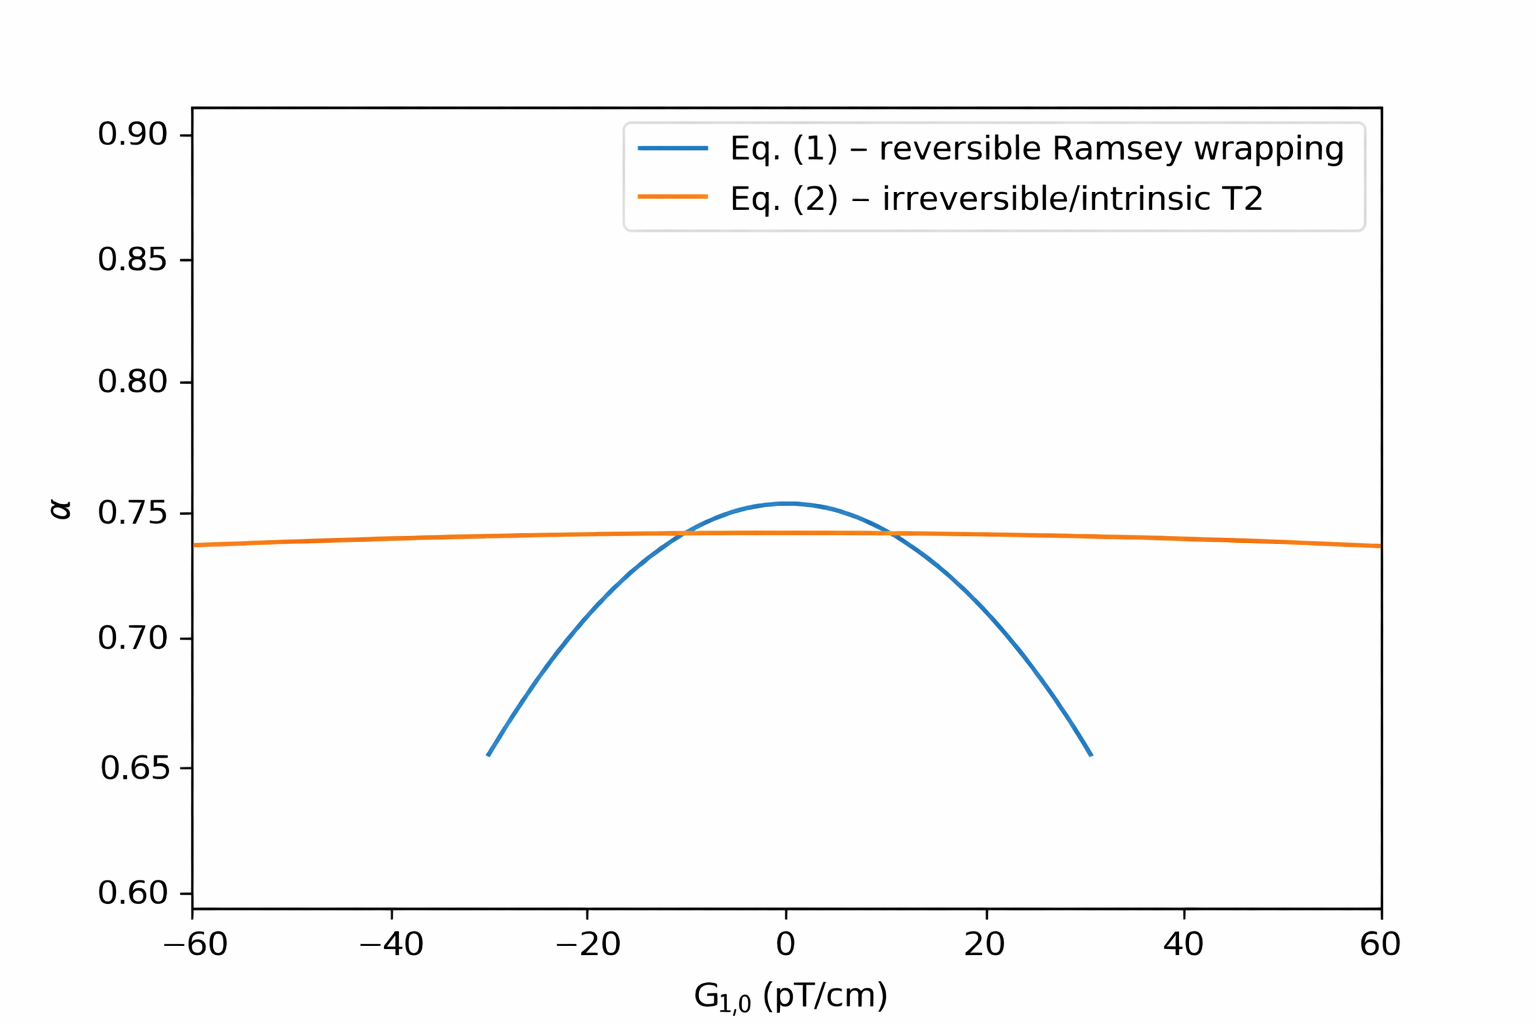
\includegraphics[width=0.78\linewidth]{Fig1Gravitational2.png}
  \caption{Calculated neutron visibility $\alpha$ after $T=180$~s as a function of the vertical gradient $G_{1,0}$, comparing gravitationally enhanced depolarization (reversible, ``Ramsey wrapping'') and intrinsic depolarization (irreversible). The curves are obtained from the first-order gradient model using Eqs.~(\ref{eq:grav}) and (\ref{eq:intrinsic_visibility}) with parameters taken from Ref.~\cite{bib:Abel2019}.}
  \label{fig:g10_visibility}
\end{figure}

Figure~\ref{fig:g10_visibility} shows the visibility predicted by the first-order gradient model after $T=180$~s as a function of the vertical gradient $G_{1,0}$, comparing gravitationally enhanced (reversible) and intrinsic (irreversible) depolarization. For the purposes of argument, let us adopt a goal of
\begin{equation}
  T_2>10{,}000~{\rm s}.
  \label{eq:t2goal}
\end{equation}
This would correspond to visibility at $T=180$~s of
\begin{equation}
  \alpha>\alpha_0\exp(-T/T_2)=\alpha_0\times 0.982.
  \label{eq:alphagoal}
\end{equation}
Using TUCAN-like cell dimensions in the same first-order gradient framework \cite{bib:MartinT2Note2020}, the requirements on the first-order gradients are summarized in Tables~\ref{tab:g10} and \ref{tab:g11}.

\begin{table}[tbp]
\centering
\small
\setlength{\tabcolsep}{4pt}
\renewcommand{\arraystretch}{1.1}
\caption{Gravitational and intrinsic depolarization constraints on best achieved $G_{1,0}$.}
\label{tab:g10}
\begin{tabular}{lcc}
\hline
 & \multicolumn{2}{c}{$G_{1,0}$ bound (pT/cm)} \\
geometry & gravitational & intrinsic \\
\hline
PSI & $< 11.7$ & $< 91.0$ \\
TUCAN each cell & $< 8.7$ & $< 58.5$ \\
TUCAN encompassing both & $< 3.4$ & $< 14.8$ \\
\hline
\end{tabular}
\end{table}

\begin{table}[tbp]
\centering
\small
\setlength{\tabcolsep}{4pt}
\renewcommand{\arraystretch}{1.1}
\caption{Intrinsic depolarization constraints on best achieved $\sqrt{G_{1,1}^2+G_{1,-1}^2}$.}
\label{tab:g11}
\begin{tabular}{lc}
\hline
geometry & upper bound (pT/cm) \\
\hline
PSI & $< 15.6$ \\
TUCAN each cell & $< 10.8$ \\
TUCAN encompassing both & $< 10.8$ \\
\hline
\end{tabular}
\end{table}

Table~\ref{tab:g11} displays the requirement on transverse gradients of $B_z$. Equation~(\ref{eq:intrinsic_visibility}) has been used with $G_{1,0}$ set to zero. The gradient should be less than 11~pT/cm for TUCAN, if an $R=0.3$ cell is used. The constraint does not depend on the cell height. Table~\ref{tab:g10} displays requirements on the vertical gradient of $B_z$ to achieve a long neutron $T_2$. The most stringent constraint arises due to taller cells \cite{bib:MartinT2Note2020}. For higher-order gradients, it is important to perform some kind of averaging over the cell. A recommendation for a general field $B_z(x,y,z)$ is to require
\begin{equation}
  \Delta B_z=B_z^{\rm max}-B_z^{\rm min}<G_{1,0}^{\rm goal}H,
\end{equation}
where the maximum and minimum are determined within the measurement cell. Another measure of the variation in $B_z$ could alternately be used, for example:
\begin{equation}
  \sigma(B_z)<\frac{G_{1,0}^{\rm goal}H}{\sqrt{12}}.
\end{equation}
Likewise, we can estimate a constraint arising from transverse gradients could be
\begin{equation}
  \Delta B_z=B_z^{\rm max}-B_z^{\rm min}<2G_{1,1}^{\rm goal}R
\end{equation}
or, if using the standard deviation to set the constraint,
\begin{equation}
  \sigma(B_z)<\frac{G_{1,1}^{\rm goal}R}{2}.
\end{equation}
If these constraints are adopted, the tightest constraint on the $B_z$ variation always arises due to the gravitational depolarization constraints on $G_{1,0}$. Multiplying by the height of the cell gives the requirement $G_{1,0}H<G_{1,0}^{\rm goal}H=140$~pT. This would imply the following suggested constraints on our $B_z$-variation metrics \cite{bib:MartinT2Note2020}:
\begin{equation}
  \Delta B_z<140~{\rm pT}\qquad\text{or}\qquad\sigma(B_z)<40~{\rm pT}.
  \label{eq:bzmetrics}
\end{equation}
These requirements should be applied to the square shim coil design. These requirements could be argued to be too stringent for the square shim coils by a factor of 10 \cite{bib:MartinT2Note2020}. We plan to have excellent $G_{\ell,0}$ coils in addition to the square shims. These will be designed to control false EDM effects, and to apply pure $G_{\ell,0}$ fields \cite{bib:MartinT2Note2020}.

Transverse fields affect the comparison of the comagnetometer frequency, which senses $B_z$, to the neutron frequency, which senses $|\vec{B}|$. To lowest order, they differ by $\frac{\langle B_T^2\rangle}{2B_0^2}$ \cite{bib:Abel2019}. In the PSI nEDM experiment, typically $\langle B_T^2\rangle\sim 1$~nT$^2$ was achieved. Since TUCAN aims to measure the precession frequency with a factor of ten better precision, a sufficient goal for TUCAN would be \cite{bib:MartinT2Note2020}
\begin{equation}
  \langle B_T^2\rangle<0.1~{\rm nT}^2.
  \label{eq:bt2goal}
\end{equation}
As acknowledged in Ref.~\cite{bib:Abel2019}, this is normally achieved if the $B_z$ homogeneity is achieved (by orders of magnitude).

\section{Design concept}\label{sec3}

The square shim coils provide flexible control of magnetic-field inhomogeneities inside the magnetically shielded room (MSR), complementing the main holding-field coil. In TUCAN, the shim system is used both to improve field homogeneity in the measurement region (supporting long neutron-$T_2$) and to deliberately generate specific gradient modes for systematic studies. This section summarizes the coil layout and the current-supply approach used to drive the multi-coil array.

\subsection{Coil geometry and operating range}

The coils are arranged on the faces of a cube that defines the winding surface. A common baseline uses a $3\times3$ grid of square coils per face, giving $9\times6=54$ coils in total. Field quality is evaluated in a smaller inner region of interest (ROI), represented by a grid of points (or sensor locations) inside the cube. Figure~\ref{fig:shim_geometry} shows an example geometry used for design studies and for constructing the response matrix described in Section~\ref{sec:matrixmethods}.

\begin{figure}[tbp]
  \centering
  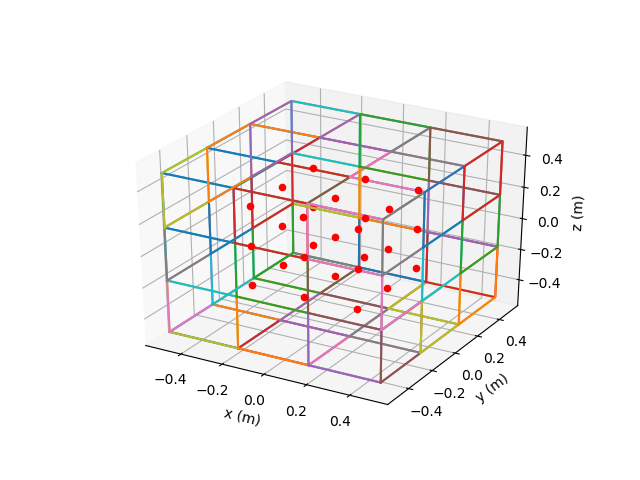
\includegraphics[width=0.82\linewidth]{Fig2example-geometry.png}
  \caption{Example square-shim geometry: nine coils on each of six faces (54 coils total) and a representative set of points in the inner ROI used for field evaluation and matrix construction.}
  \label{fig:shim_geometry}
\end{figure}

The required current per channel is modest (typically tens of mA), but stability and reproducibility are important because current drifts translate directly into field drifts. For prototype and commissioning work, we therefore use independent bipolar channels with a full-scale capability of approximately $\pm 40$~mA per channel.

\subsection{Multi-channel current supply}

Independent control of the shim-coil array is provided by a modular 64-channel bipolar supply: one power/distribution board plus four identical 16-channel current-source boards (Fig.~\ref{fig:cs_shim_pcb}). This provides margin beyond the 54-coil baseline configuration and allows each coil to be driven with an independent, reproducible current. Digital setpoints are produced by an Arduino on the power/distribution board and sent to the four current-source boards via SPI. The MOSI, MISO, and SCK lines are shared, and each 16-channel board is addressed using a dedicated chip-select line; pull-up resistors on the chip-select lines help ensure defined logic levels during communication. Each current-source board receives both power and control signals through a multi-pin connector.

Each current-source board uses a 16-channel, 16-bit DAC (LTC2668) that provides a programmable reference voltage up to $\pm 10$~V per channel. The output current is regulated using a precision sense resistor in a stabilized feedback loop (Fig.~\ref{fig:cs_shim_pcb}b). In the channel architecture, an instrumentation amplifier in the feedback path (gain 50) forces the voltage across the sense resistor to track the programmed reference. With $V_{\mathrm{ref}}=\pm 10$~V and $R_S=5~\Omega$, the full-scale current is approximately $\pm 40$~mA. A small compensation network is included to damp oscillations and improve stability when driving inductive loads such as the shim coils.

\begin{figure}[tbp]
  \centering
  \begin{minipage}[t]{0.39\textwidth}
    \centering
    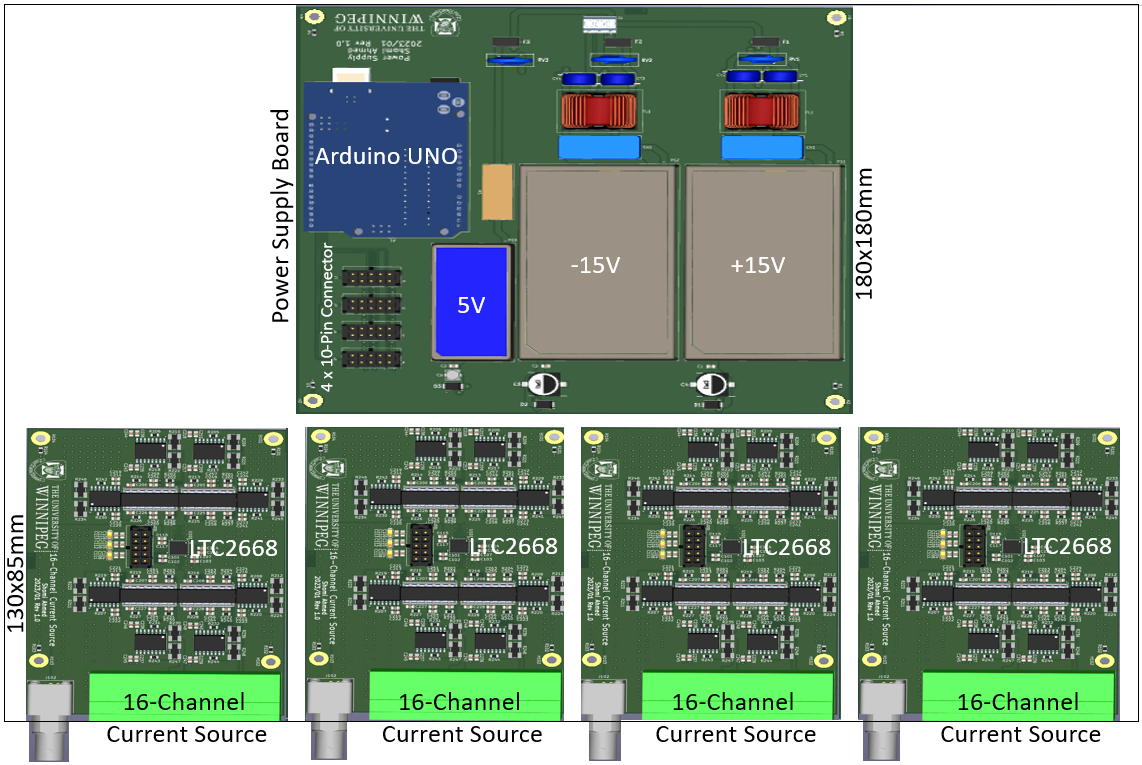
\includegraphics[width=\linewidth]{Fig3cs_shim_pcb.png}
    \vspace{1mm}
    {\scriptsize (a)}
  \end{minipage}\hfill
  \begin{minipage}[t]{0.57\textwidth}
    \centering
    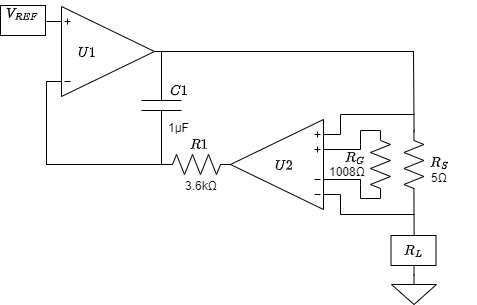
\includegraphics[width=\linewidth]{Fig3acs_shim.png}
    \vspace{1mm}
    {\scriptsize (b)}
  \end{minipage}
  \caption{Modular 64-channel shim-coil current supply. (a) Power/distribution board and four 16-channel current-source boards. (b) One-channel schematic showing the programmable reference voltage, precision sense resistor, and stabilized feedback loop used to generate a controlled bipolar output current.}
  \label{fig:cs_shim_pcb}
\end{figure}

\section{Matrix methods}\label{sec:matrixmethods}

The square shim system is operated using a matrix-based setpoint calculation: a linear response matrix is built for the coil array and a pseudoinverse is used to find the coil currents that best realize a desired field pattern in a region of interest (ROI). The method also exposes a singular ``zero mode'' that must be removed for numerical stability \cite{bib:klassen2026squares}.

\subsection{Linear response matrix}

Consider $c$ independently driven coils, labeled by $j=1,\dots,c$, with currents collected into a vector $I=(I_1,\dots,I_c)^T$. The magnetic field is evaluated at $N$ locations in the ROI using three-axis sensors (or an equivalent set of evaluation points). We stack the measured components into a single vector $B=(B_1,\dots,B_s)^T$, where $s=3N$ if all components $(B_x,B_y,B_z)$ are used.

For a fixed geometry, the field at each sensor axis is linear in the coil currents,
\begin{equation}
  B_i=\sum_{j=1}^{c} M_{ij} I_j,
  \label{eq:Bij}
\end{equation}
where $M_{ij}$ is the field produced at axis $i$ per unit current in coil $j$. In matrix form,
\begin{equation}
  B=MI.
  \label{eq:forward_matrix}
\end{equation}
In free-space studies, the elements of $M$ can be computed using a Biot--Savart model for each square coil treated as a set of straight segments \cite{bib:klassen2026squares,bib:freespacecode}. For MSR-coupled operation, $M$ can alternatively be generated from magnetostatic finite-element simulations that include the surrounding magnetic materials and geometry \cite{bib:comsol}.

\subsection{Setpoint calculation with the pseudoinverse}

Given a target field vector $B_{\mathrm{target}}$ defined on the same ROI grid, the desired coil currents are obtained by solving the inverse problem. In general the system is overdetermined ($s>c$) and we seek the least-squares solution,
\begin{equation}
  I_{\mathrm{set}}=M^{+}B_{\mathrm{target}},
  \label{eq:setpoints}
\end{equation}
where $M^{+}$ is the Moore--Penrose pseudoinverse.

We compute $M^{+}$ using a singular value decomposition (SVD),
\begin{equation}
  M=USV^{T},
  \label{eq:svd}
\end{equation}
where $U$ is an $s\times s$ orthogonal matrix, $V$ is a $c\times c$ orthogonal matrix, and $S$ is an $s\times c$ diagonal matrix whose diagonal entries $S_{ii}$ are non-negative singular values ordered from largest to smallest. Defining a diagonal matrix $D$ with elements
\begin{equation}
  D_{ii}=\frac{1}{S_{ii}},
  \label{eq:Ddef}
\end{equation}
the pseudoinverse is constructed as
\begin{equation}
  M^{+}=VS^{+}U^{T},
  \qquad
  S^{+}=D^{T},
  \label{eq:pinv_svd}
\end{equation}
and used in Eq.~(\ref{eq:setpoints}) to compute $I_{\mathrm{set}}$ \cite{bib:klassen2026squares}.

\subsection{Zero mode and truncation}

For square coils with overlapping currents inscribed on a closed cube, there exists a singular ``zero mode'': applying equal-magnitude current to all coils produces zero net current and therefore generates $B\approx 0$ everywhere. In the SVD this appears as a vanishing (or numerically tiny) smallest singular value,
\begin{equation}
  S_{cc}\approx 0,
\end{equation}
which would make $D_{cc}=1/S_{cc}$ diverge and destabilize the inversion \cite{bib:klassen2026squares}.

We remove this mode using truncation. Concretely, we omit the final singular value and its associated singular vectors when forming the inverse. Let $S'$ denote $S$ with its last (smallest) singular value removed, and let $V'$ denote $V$ with the corresponding singular vector removed. The truncated pseudoinverse becomes
\begin{equation}
  M^{+}_{\mathrm{trunc}}=V'(S')^{+}U^{T},
  \label{eq:pinv_trunc}
\end{equation}
and the stable setpoints are
\begin{equation}
  I_{\mathrm{set}}=M^{+}_{\mathrm{trunc}}B_{\mathrm{target}}.
\end{equation}
This procedure preserves the physically meaningful modes while suppressing the singular current pattern that produces no field.

\subsection{Target fields for optimization and systematic modes}

The target vectors $B_{\mathrm{target}}$ are generated either as (i) corrections to reduce inhomogeneity metrics such as $\Delta B_z$ and $\sigma(B_z)$ (Section~\ref{sec2}), or as (ii) specific gradient modes $G_{\ell,m}$ used for systematic studies. Once $I_{\mathrm{set}}$ is computed, the achieved field is evaluated using the same ROI metrics and compared against the design goals and against mapping measurements (Section~\ref{sec7}).

\section{Evolution of the shim coil design}\label{sec5}

Design work for TUCAN shimming has explored how to generate controlled harmonic modes while limiting sensitivity to magnetic materials and maintaining practical access within the MSR. A key design driver is the degree of coupling between the shim coils and the innermost magnetic shield \cite{bib:martin2026options}.

\subsection{Design options: self-shielded and shield-coupled coils}

Three broad approaches have been considered \cite{bib:martin2026options}. In a self-shielded design, coils are wound on two surfaces (inner and outer) so that the external field cancels while the desired field is produced inside the inner surface. This avoids magnetic materials in the design model, but requires additional space and complicates access because two winding surfaces must be accommodated.

A tightly shield-coupled design winds coils on (or near) a nearly closed mu-metal flux return, such as the innermost shield or a dedicated yoke. This can simplify the analytic form of some modes, but it maximizes coupling to the shield and can increase sensitivity to penetrations, non-ideal shield joints, and assembly details of the MSR.

A slightly shield-coupled design places coils on an inner winding surface (for example, near the vacuum enclosure or an engineered frame) while explicitly accounting for the shield response in the design model. This approach avoids the need for a second winding surface and reduces dependence on shield properties compared to the tightly coupled case, while remaining compatible with numerical design tools \cite{bib:martin2026options,bib:comsol}. For TUCAN, this compromise provides a practical balance between mechanical simplicity and predictable magnetic performance.

\subsection{Square shim coils and matrix-designed setpoints}

To provide flexible control over a wide range of inhomogeneity patterns, TUCAN has adopted square-coil arrays on panelized cubic faces. This architecture supports many independent channels and is naturally compatible with matrix-designed setpoints (Section~\ref{sec:matrixmethods}). Design studies show that a $3\times3$ array on each face (54 coils total) provides enough degrees of freedom to address $B_z$ inhomogeneity targets in an ROI, while keeping current requirements modest \cite{bib:klassen2026squares}. In the present implementation, currents are computed from a response matrix using an SVD-based pseudoinverse with the singular zero mode removed \cite{bib:klassen2026squares}.

Figure~\ref{fig:squares_demo} shows an example of this workflow for a $G_{1,0}=1$ target field: the achieved field follows the target structure and the residual field is strongly suppressed within the ROI after applying the matrix-derived setpoints. This type of validation is useful during design iteration and provides an intuitive link between the matrix formalism and the mapping measurements discussed later in Section~\ref{sec7}.

\begin{figure}[tbp]
  \centering
  \begin{minipage}[t]{0.48\textwidth}
    \centering
    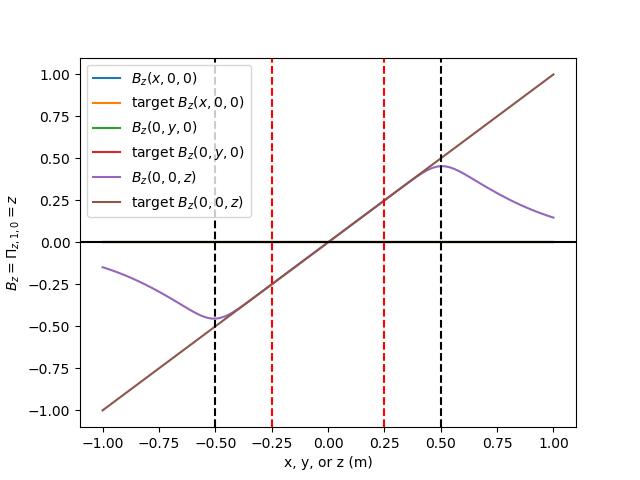
\includegraphics[width=\linewidth]{Fif4ag10-z.png}
    \vspace{1mm}
    {\scriptsize (a)}
  \end{minipage}\hfill
  \begin{minipage}[t]{0.48\textwidth}
    \centering
    \includegraphics[width=\linewidth]{g10-z-residual.png}
    \vspace{1mm}
    {\scriptsize (b)}
  \end{minipage}
  \caption{Matrix-method example for a $G_{1,0}=1$ target field: (a) target and coil-generated $B_z$ evaluated along the coordinate axes; (b) residual $B_z$ (coil-generated minus target). Vertical black dashed lines indicate the extent of the coil cube and red dashed lines indicate the fluxgate scan range.}
  \label{fig:squares_demo}
\end{figure}

\subsection{ROI performance metrics}

A convenient summary of shim performance is obtained by evaluating homogeneity metrics within an ROI before and after applying correction currents. Table~\ref{tab:roi_metrics} lists representative values of $\Delta B_z$, $\sigma(B_z)$, and $\langle B_T^2\rangle$ for several target fields, together with the extrema of the required coil currents \cite{bib:katotoka2025}. The table includes dipole-like perturbations and selected $(\ell,m)$ modes. In general, the residual values of $\Delta B_z$ and $\sigma(B_z)$ are substantially reduced after correction and are compatible with the variations goals of $B_z$ discussed in Section~\ref{sec2}, while the required currents remain at the few--to-few$\times10$~mA scale.

\begin{table}[tbp]
\centering
\scriptsize
\setlength{\tabcolsep}{3pt}
\renewcommand{\arraystretch}{1.05}
\resizebox{\textwidth}{!}{%
\begin{tabular}{lrrrrrrrr}
\hline
\multirow{2}{*}{\shortstack{$(l,m)$\\ or\\ dipole}} &
\multicolumn{2}{c}{\shortstack{$\Delta B_z$\\(pT)}} &
\multicolumn{2}{c}{\shortstack{$\sigma(B_z)$\\(pT)}} &
\multicolumn{2}{c}{\shortstack{$\langle B_T^2\rangle$\\(nT$^2$)}} &
\multirow{2}{*}{\shortstack{max current\\(A)}} &
\multirow{2}{*}{\shortstack{min current\\(A)}} \\
\cmidrule(lr){2-3}\cmidrule(lr){4-5}\cmidrule(lr){6-7}
 & \shortstack{before\\correction} & \shortstack{after\\correction}
 & \shortstack{before\\correction} & \shortstack{after\\correction}
 & \shortstack{before\\correction} & \shortstack{after\\correction}
 & & \\
\hline
(1,0)          & 1200 & 14   & 394 & 0.3 & 0.26   & 0                & 0.005020 & -0.006836 \\
(1,1)          & 1740 & 18   & 448 & 2   & 0.36   & $1\times10^{-5}$ & 0.013633 & -0.013633 \\
(2,0)          & 500  & 5    & 105 & 0.6 & 0.04   & $1\times10^{-6}$ & 0.012787 & -0.012787 \\
(2,1)          & 696  & 6    & 118 & 1   & 0.02   & $2\times10^{-6}$ & 0.009073 & -0.009073 \\
(2,2)          & 1009 & 22   & 218 & 2   & 0.16   & $3\times10^{-5}$ & 0.015374 & -0.015374 \\
dipole 1       & 1060 & 33   & 226 & 2   & 0.40   & $2\times10^{-5}$ & 0.026277 & -0.026277 \\
dipole 2 upper & 509  & 0.7  & 111 & 0.1 & 0.44   & 0                & 0.001914 & -0.017904 \\
dipole 2 lower & 208  & 1    & 47  & 0.1 & 0.44   & 0                & 0.001914 & -0.017904 \\
dipole 3 upper & 852  & 11   & 181 & 2   & 0.15   & $4\times10^{-6}$ & 0.015423 & -0.015423 \\
dipole 3 lower & 852  & 11   & 181 & 2   & 0.15   & $4\times10^{-6}$ & 0.015423 & -0.015423 \\
\hline
goal           &      & 140  &      & 40  &        & 0.1              &          &          \\
\hline
\end{tabular}%
}
\caption{Representative ROI performance metrics before and after matrix-based correction for selected target fields, together with the extrema of the required coil currents.}
\label{tab:roi_metrics}
\end{table}

\section{Construction and installation}\label{sec6}

\subsection{Panel fabrication and coil winding}

The shim-coil array was implemented on a $4'\times4'$ corrugated plastic (Coroplast) sheet, chosen because it is lightweight, rigid, and easy to machine and handle. The coil geometry was marked directly on the sheet using simple layout tools (e.g., T-square/carpenter’s square and measuring tapes), and squareness was checked by comparing measured diagonals to the expected values. After the layout was verified, grooves were cut to guide the wire placement: grooves across the ribs were made using a thin circular-saw blade, while grooves along the ribs were made using a knife.

Each square coil was wound using 30~AWG magnet wire with three turns per coil, which provides sufficient field amplitude at modest operating currents. On each panel, the lead wires were routed so that they converge at a common exit point, simplifying cable organization and reducing clutter inside the MSR. Where necessary, small cut-outs were made in the panel patterns to accommodate MSR structural extrusions while keeping the coil paths continuous.

\subsection{Installation inside the MSR and cabling}

The completed panels were installed on the inner MSR walls and secured using a simple mounting approach (mechanical fastening where available, supplemented by tape) to keep the panels stable while still allowing removal and replacement during MSR access. The six faces were labeled by wall (east, west, north, south, floor, ceiling) and the coils/connectors were numbered consistently so that software-defined current setpoints map to the correct physical coils.

For each face, nine coils require eighteen conductors (two leads per coil). Ethernet cables were used as convenient multi-conductor bundles, with three cables per face and all cables routed through the MSR extrusions to a centralized location for easier connection to the current source. This organized routing and labeling is essential for reliable commissioning, mapping, and repeatable generation of harmonic modes.

\begin{figure}[tbp]
  \centering
  \includegraphics[width=0.68\linewidth]{Fig5.png}
  \caption{Prototype square shim coils installed inside the TUCAN MSR. The system comprises 54 coils (nine coils on each of the six faces). The MSR provides passive magnetic shielding using high-permeability mu-metal.}
  \label{fig:msr_prototype_install}
\end{figure}

\section{Mapping results}\label{sec7}

Magnetic field mapping of the shim coil system was carried out inside the magnetically shielded room to verify proper coil operation and to evaluate the ability of the system to generate controlled magnetic field gradients required for the TUCAN neutron electric dipole moment experiment. Mapping measurements were performed along a central scan axis using a three-axis fluxgate magnetometer, and the magnetic field components $B_x$, $B_y$, and $B_z$ were recorded at each scan position.

\subsection{Verification of individual shim coils}

As a first step, each of the 54 shim coils was individually mapped to verify the proper electrical connection and magnetic response. At each position along the scan axis, a current of $+40~\mathrm{mA}$ was applied to a single coil and the magnetic field components $B_x$, $B_y$, and $B_z$ were measured. The current was then reversed to $-40~\mathrm{mA}$ and the measurement was repeated. The difference between the two measurements isolates the magnetic field generated by the coil while reducing the effect of background magnetic fields and slow drifts.

All individual coil scans show smooth and reproducible magnetic field profiles. No missing or abnormal coil responses were observed. A representative single-coil scan is shown in Fig.~\ref{fig:singlecoil}. These results confirm that all shim coils are functioning as expected and are suitable for producing controlled magnetic field gradients.

\begin{figure}[tbp]
  \centering
  \includegraphics[width=0.92\linewidth]{Fig6singleall.png}
  \caption{Magnetic field components $B_x$, $B_y$, and $B_z$ measured along the scan axis for a representative shim coil using $\pm 40~\mathrm{mA}$ current. The difference between the $+I$ and $-I$ measurements isolates the coil field and confirms proper coil operation.}
  \label{fig:singlecoil}
\end{figure}

\subsection{Mapping of the $G_{1,0}$ harmonic mode}

After verifying the individual coils, the shim coil system was configured to generate the lowest-order gradient mode $G_{1,0}$. The set points of the coil current were calculated using two methods. In the first method, analytic free space calculations were used, assuming that there are no surrounding magnetic materials \cite{bib:freespacecode}. In the second method, coil response matrices were obtained using finite-element simulations with COMSOL Multiphysics, which include the effect of the magnetically shielded room \cite{bib:comsol}.

Magnetic field maps for the $G_{1,0}$ mode were recorded along the central scan axis using custom Python-based data acquisition and analysis software \cite{bib:mappingcode}. The measured magnetic field components $B_x$, $B_y$, and $B_z$ show good agreement in spatial shape with the simulated fields. Figure~\ref{fig:G10map} shows the measured and simulated field components. A difference in overall field amplitude between measurement and simulation was observed and corrected by applying a single normalization factor derived from the $B_x$ component.

\begin{figure}[tbp]
  \centering
  \includegraphics[width=0.92\linewidth]{G10shim.png}
  \caption{Measured and simulated magnetic field components $B_x$, $B_y$, and $B_z$ along the central scan axis for the $G_{1,0}$ gradient mode. The measured fields are compared with COMSOL-based simulations using the same current setpoints. A single scaling factor is applied to the simulated field to account for the overall amplitude difference.}
  \label{fig:G10map}
\end{figure}

After normalization, the residual magnetic field, defined as the difference between the measured field and the scaled simulated field, was reduced to approximately $\pm 0.5~\mathrm{nT}$ over the region of interest. The residual fields for the $G_{1,0}$ mode are shown in Figure~\ref{fig:G10residual}. These results demonstrate that the shim coil system can reliably generate and control the dominant vertical gradient field.

\begin{figure}[tbp]
  \centering
  \includegraphics[width=0.82\linewidth]{G10 residual shim.png}
  \caption{Residual magnetic field for the $G_{1,0}$ gradient mode along the central scan axis after normalization of the simulated field to the measured field.}
  \label{fig:G10residual}
\end{figure}

\subsection{Generation of higher-order harmonic modes}

In addition to the $G_{1,0}$ mode, the shim coil system was used to generate higher-order harmonic modes, including $G_{1,2}$ and $G_{2,1}$. For these measurements, the coil current setpoints were calculated using COMSOL-based response matrices. Magnetic field profiles measured along the central scan axis for these modes are shown in Fig.~\ref{fig:residuals_G12_G21}.

\begin{figure}[tbp]
  \centering
  \begin{minipage}[t]{0.86\textwidth}
    \centering
    \includegraphics[width=\linewidth]{G12 shim.png}
    \vspace{1mm}

    {\small (a) $G_{1,2}$}
  \end{minipage}

  \vspace{3mm}

  \begin{minipage}[t]{0.86\textwidth}
    \centering
    \includegraphics[width=\linewidth]{G21shim.png}
    \vspace{1mm}

    {\small (b) $G_{2,1}$}
  \end{minipage}
  \caption{Measured and COMSOL-simulated magnetic field components $B_x$, $B_y$, and $B_z$ along the central scan axis for the $G_{1,2}$ and $G_{2,1}$ gradient modes generated using COMSOL-derived current setpoints. The panels are stacked vertically to preserve readable axis labels and legends at the manuscript submission size.}
  \label{fig:residuals_G12_G21}
\end{figure}

The measured field shapes for the higher-order modes follow the expected spatial structure of the corresponding harmonic fields. These measurements demonstrate the flexibility of the shim coil system and its capability to generate a range of gradient field configurations relevant for magnetic field optimization in the TUCAN nEDM experiment. A detailed quantitative analysis of higher-order modes is left for future work.

\section{Discussion and Conclusion}\label{sec8}

The magnetic field mapping results demonstrate that the square shim coil system can reliably generate controlled gradient fields inside the magnetically shielded room for the TUCAN nEDM experiment. Central-axis scans of the three field components provide a direct validation of the coil response and of the current setpoints used for field generation.

For the $G_{1,0}$ configuration, the measured field components $B_x$, $B_y$, and $B_z$ reproduce the simulated spatial structure along the scan axis. An overall amplitude difference between measurement and simulation was accounted for using a single normalization factor derived from the $B_x$ component, and the residual field after normalization is reduced to approximately $\pm 0.5~\mathrm{nT}$ over the region of interest. These results show that the shim coil system can generate and tune the dominant vertical gradient field required for field optimization.

Higher-order harmonic modes were also generated using COMSOL-derived current setpoints. The measured profiles follow the expected harmonic structure and remain consistent with the simulated field components along the central scan axis, demonstrating the flexibility of the shim coil system and its capability to produce a range of gradient-field configurations relevant for magnetic field optimization in the TUCAN nEDM experiment.

Future work will extend this characterization beyond the central axis by analyzing field maps acquired in additional mapping holes and through the MSR door, and by carrying out a more detailed quantitative evaluation of higher-order mode performance, repeatability, and stability.

\section*{Acknowledgements}

% Add your acknowledgements here.

\bibliographystyle{elsarticle-num}
\bibliography{shim_coil_refs}

\end{document}